\chapter{CMB Lensing Remapping, Lensing \texorpdfstring{$B$}{B} Modes, and Cross-Observable Scale Separation}
\label{ch:cmb-lensing-remapping}

\section{Scope and objective}

The production-to-CMB calculation supplies controlled unlensed $TT$, $TE$, and $EE$ templates, while the collisionless refinement calculation supplies a late-time scale-dependent matter transfer.  The missing linear-observable link was the gravitational remapping between them.  This chapter constructs a common lensing potential, remaps the temperature and polarization fields without retuning the dark sector, generates the scalar lensing $B$ mode, and compares the resulting CMB response with the previously computed galaxy-lensing response.

The result is a controlled Born, flat-sky, Gaussian-remapping benchmark.  It is not a precision CMB-lensing likelihood.  The matter spectrum is normalized to a declared $\sigma_8$ benchmark, its smooth baseline transfer omits baryon wiggles, and nonlinear matter power, post-Born corrections, foregrounds, and delensing are not included.

\section{Matter spectrum and fixed refinement transfer}

Let
\begin{equation}
 \Omega_{m0}=\Omega_{b0}+\Omega_{D0}=0.310,
 \qquad
 \Omega_{r0}=9.0\times10^{-5},
 \qquad
 \Omega_{V0}=1-\Omega_{m0}-\Omega_{r0}.
 \label{eq:lens-background-fractions}
\end{equation}
The background is
\begin{equation}
 E(a)^2=\Omega_{r0}a^{-4}+\Omega_{m0}a^{-3}+\Omega_{V0}.
 \label{eq:lens-background}
\end{equation}
A smooth control matter spectrum is written
\begin{equation}
 P_{\rm c}(k,0)=A_P k^{n_s}T_{\rm sm}(k)^2,
 \label{eq:lens-control-power}
\end{equation}
where the amplitude $A_P$ is fixed by
\begin{equation}
 \sigma_8^2
 =\int_0^\infty \frac{k^3P_{\rm c}(k,0)}{2\pi^2}
 W_{\rm TH}(kR_8)^2\,d\log k,
 \qquad
 R_8=\frac{8}{h}\ {\rm Mpc}.
 \label{eq:lens-sigma8-normalization}
\end{equation}
The deterministic calculation uses
\begin{equation}
 n_s=0.965,
 \qquad
 \sigma_8=0.81.
 \label{eq:lens-normalization-values}
\end{equation}
The refinement matter spectrum is not refitted.  It is
\begin{equation}
 P_D(k,a)=D(a)^2T_D(k)^2P_{\rm c}(k,0),
 \label{eq:lens-refinement-power}
\end{equation}
where $T_D(k)$ is the momentum-resolved collisionless transfer already derived from the scale-covariant production distribution.

\section{CMB convergence and lensing potential}

For a source plane at comoving distance $\chi_*$, define
\begin{equation}
 W_\kappa(\chi)
 =\frac{3}{2}\Omega_{m0}\left(\frac{H_0}{c}\right)^2
 \frac{\chi}{a(\chi)}\frac{\chi_*-\chi}{\chi_*}.
 \label{eq:lens-kernel}
\end{equation}
The Limber convergence spectrum is
\begin{equation}
 C_L^{\kappa\kappa}
 =\int_0^{\chi_*}\frac{d\chi}{\chi^2}
 W_\kappa(\chi)^2
 P_m\!\left(\frac{L+1/2}{\chi},a(\chi)\right).
 \label{eq:lens-kappa-spectrum}
\end{equation}
The lensing-potential spectrum is
\begin{equation}
 C_L^{\phi\phi}
 =\frac{4C_L^{\kappa\kappa}}{L^2(L+1)^2}.
 \label{eq:lens-phi-spectrum}
\end{equation}
The source distance inherited from the effective recombination calculation is
\begin{equation}
 \chi_*=13420.1231642\ {\rm Mpc}.
 \label{eq:lens-source-distance}
\end{equation}

\subsection{Positive-kernel monotonicity}

Assume
\begin{equation}
 0\leq T_D(k)\leq1.
 \label{eq:lens-transfer-order}
\end{equation}
Then the Limber kernel in \eqref{eq:lens-kappa-spectrum} is nonnegative, and therefore
\begin{equation}
 \boxed{
 C_{L,D}^{\kappa\kappa}
 \leq
 C_{L,{\rm c}}^{\kappa\kappa}
 }
 \label{eq:lens-monotonicity}
\end{equation}
for every retained $L$.  Hence
\begin{equation}
 C_{L,D}^{\phi\phi}\leq C_{L,{\rm c}}^{\phi\phi},
 \qquad
 \langle |\boldsymbol\alpha_D|^2\rangle
 \leq
 \langle |\boldsymbol\alpha_{\rm c}|^2\rangle.
 \label{eq:lens-deflection-order}
\end{equation}
This connects the small-scale matter cutoff to a definite sign in every linear lensing-power observable.

\begin{figure}[htbp]
\centering
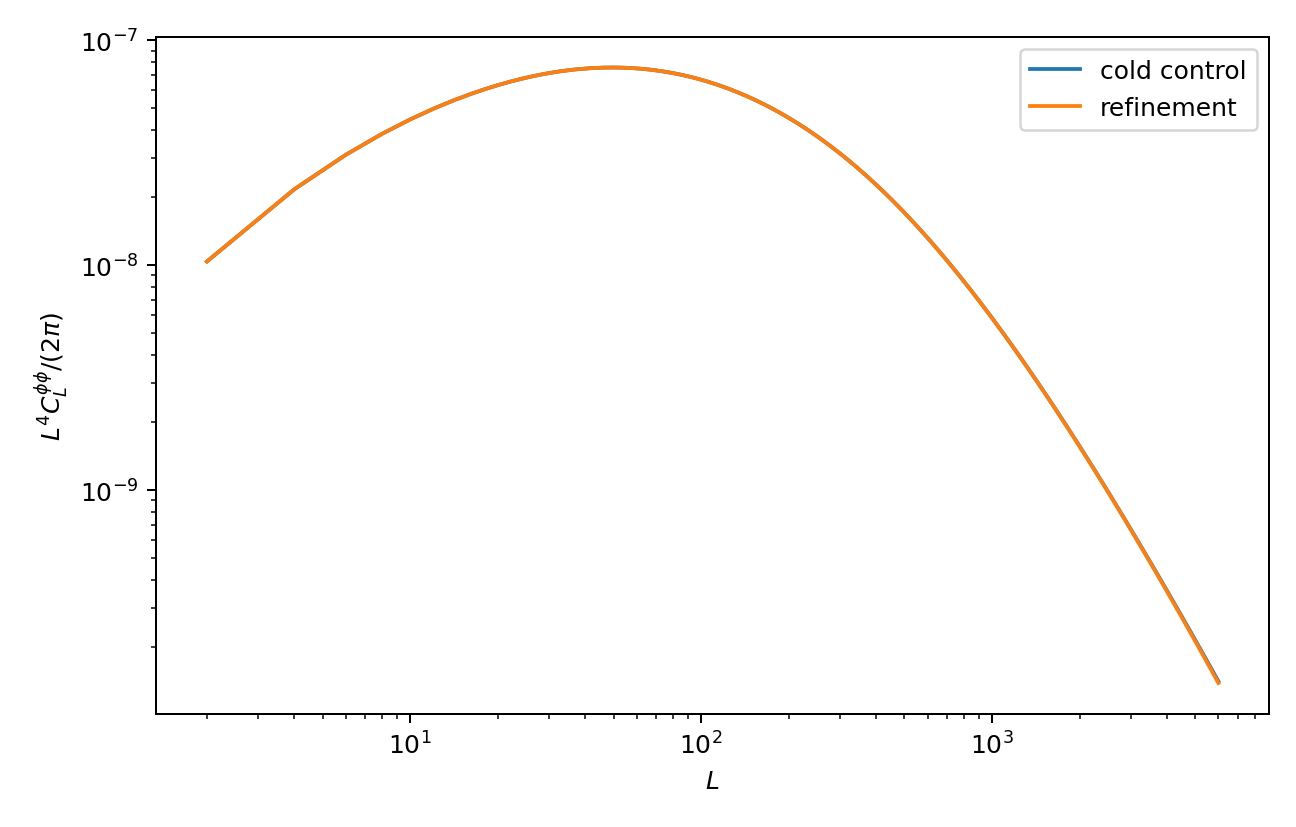
\includegraphics[width=0.86\textwidth]{figures/lens/cmb_lensing_potential.png}
\caption{The controlled CMB lensing-potential spectra.  The refinement and cold-control curves nearly coincide over the dominant CMB-lensing range because the refinement cutoff lies at substantially higher physical wavenumber.}
\label{fig:cmb-lensing-potential}
\end{figure}

\begin{figure}[htbp]
\centering
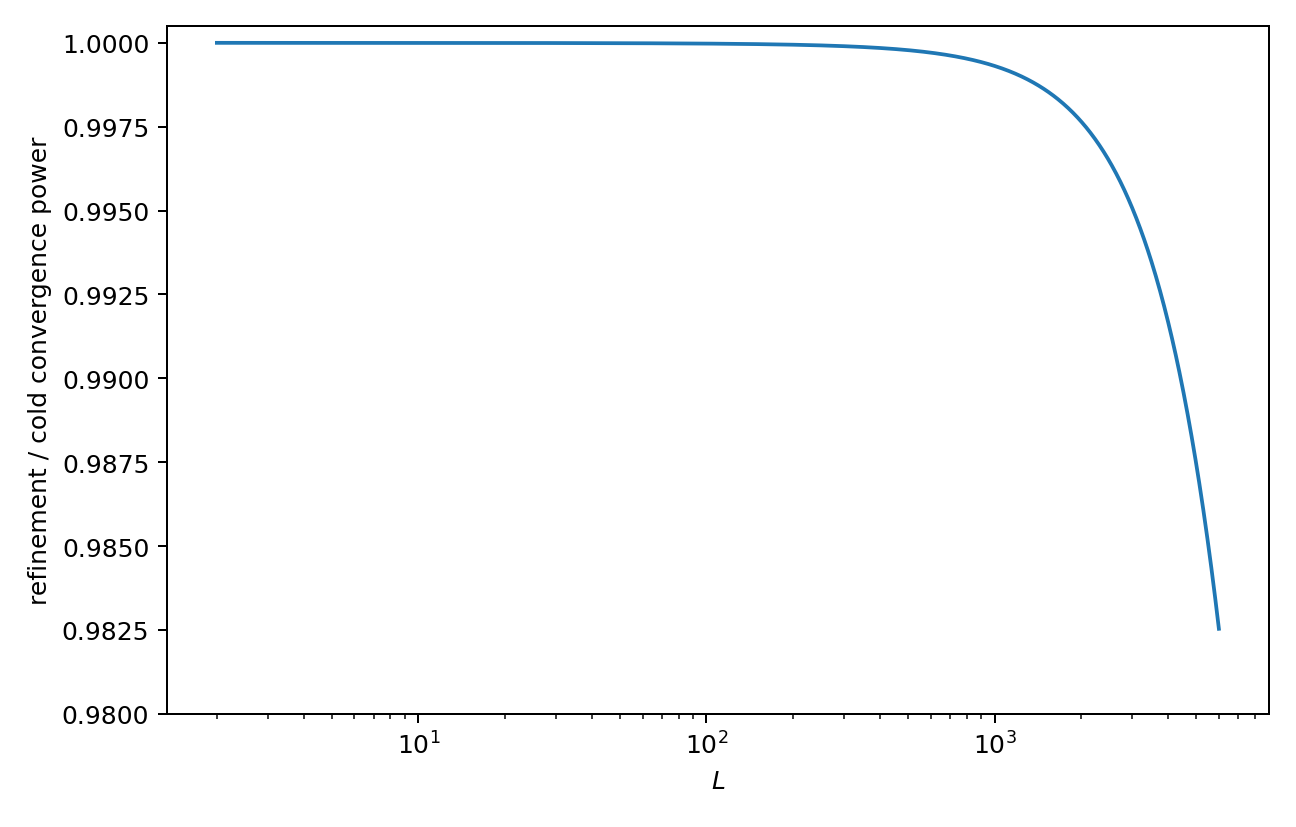
\includegraphics[width=0.82\textwidth]{figures/lens/cmb_lensing_ratio.png}
\caption{Refinement-to-cold convergence-power ratio.  The suppression grows toward high $L$, as required by the positive-kernel theorem.}
\label{fig:cmb-lensing-ratio}
\end{figure}

\section{Deflection variance and finite-patch realization}

In the continuum flat-sky normalization,
\begin{equation}
 \langle |\boldsymbol\alpha|^2\rangle
 =\int_0^\infty\frac{L^3C_L^{\phi\phi}}{2\pi}\,dL.
 \label{eq:lens-alpha-continuum}
\end{equation}
The resulting continuum rms deflections are
\begin{equation}
 \alpha_{\rm rms,c}=1.7890468022\ {\mathrm{arcmin}},
 \qquad
 \alpha_{\rm rms,D}=1.7889974544\ {\mathrm{arcmin}}.
 \label{eq:lens-alpha-values}
\end{equation}

For a periodic square of area $A$, the discrete Fourier expectation is
\begin{equation}
 \boxed{
 \langle |\boldsymbol\alpha|^2\rangle_A
 =\frac{1}{A}\sum_{\boldsymbol L}
 L^2C_L^{\phi\phi}.
 }
 \label{eq:lens-alpha-box}
\end{equation}
The principal realization uses a $20^\circ$ square, $512^2$ pixels, and forty-eight paired Gaussian realizations.  The finite box excludes the lowest deflection modes and gives
\begin{equation}
 \alpha_{\rm rms,c}^{\rm box}=1.6259829378\ {\mathrm{arcmin}},
 \qquad
 \alpha_{\rm rms,D}^{\rm box}=1.6259306696\ {\mathrm{arcmin}}.
 \label{eq:lens-alpha-box-values}
\end{equation}
The measured and discrete-expectation variances agree to $5.7\times10^{-4}$ relative accuracy.

\section{Nonperturbative map remapping}

Let $X\in\{T,Q,U\}$.  The Born remapping is
\begin{equation}
 \widetilde X(\boldsymbol n)
 =X\!\left(\boldsymbol n+\nabla\phi(\boldsymbol n)\right).
 \label{eq:lens-remap}
\end{equation}
On the flat sky,
\begin{equation}
 Q(\boldsymbol\ell)
 =E(\boldsymbol\ell)\cos2\varphi_\ell
 -B(\boldsymbol\ell)\sin2\varphi_\ell,
 \label{eq:lens-q-eb}
\end{equation}
\begin{equation}
 U(\boldsymbol\ell)
 =E(\boldsymbol\ell)\sin2\varphi_\ell
 +B(\boldsymbol\ell)\cos2\varphi_\ell.
 \label{eq:lens-u-eb}
\end{equation}
The unlensed scalar template has
\begin{equation}
 B(\boldsymbol\ell)=0.
 \label{eq:lens-unlensed-b-zero}
\end{equation}
After remapping, the inverse spin rotation produces
\begin{equation}
 \widetilde B(\boldsymbol\ell)
 =-\widetilde Q(\boldsymbol\ell)\sin2\varphi_\ell
 +\widetilde U(\boldsymbol\ell)\cos2\varphi_\ell,
 \label{eq:lens-generated-b}
\end{equation}
which is nonzero even though the primordial scalar $B$ mode vanishes.

The same primary Gaussian realization and the same lensing phases are used for the cold and refinement runs.  This paired design isolates the small difference generated by $T_D(k)$ from Monte Carlo variance.

\section{Remapped temperature and polarization}

The remapping smooths the acoustic pattern.  Around the second temperature peak, the declared peak-to-neighboring-trough contrast changes from
\begin{equation}
 \mathcal C_2^{\rm unlensed}=0.4493968827
 \label{eq:lens-contrast-unlensed}
\end{equation}
to
\begin{equation}
 \mathcal C_2^{\rm lensed}=0.4382775755.
 \label{eq:lens-contrast-lensed}
\end{equation}
Thus
\begin{equation}
 \boxed{
 \frac{\mathcal C_2^{\rm lensed}}
 {\mathcal C_2^{\rm unlensed}}
 =0.9752572669<1.
 }
 \label{eq:lens-contrast-ratio}
\end{equation}

\begin{figure}[htbp]
\centering
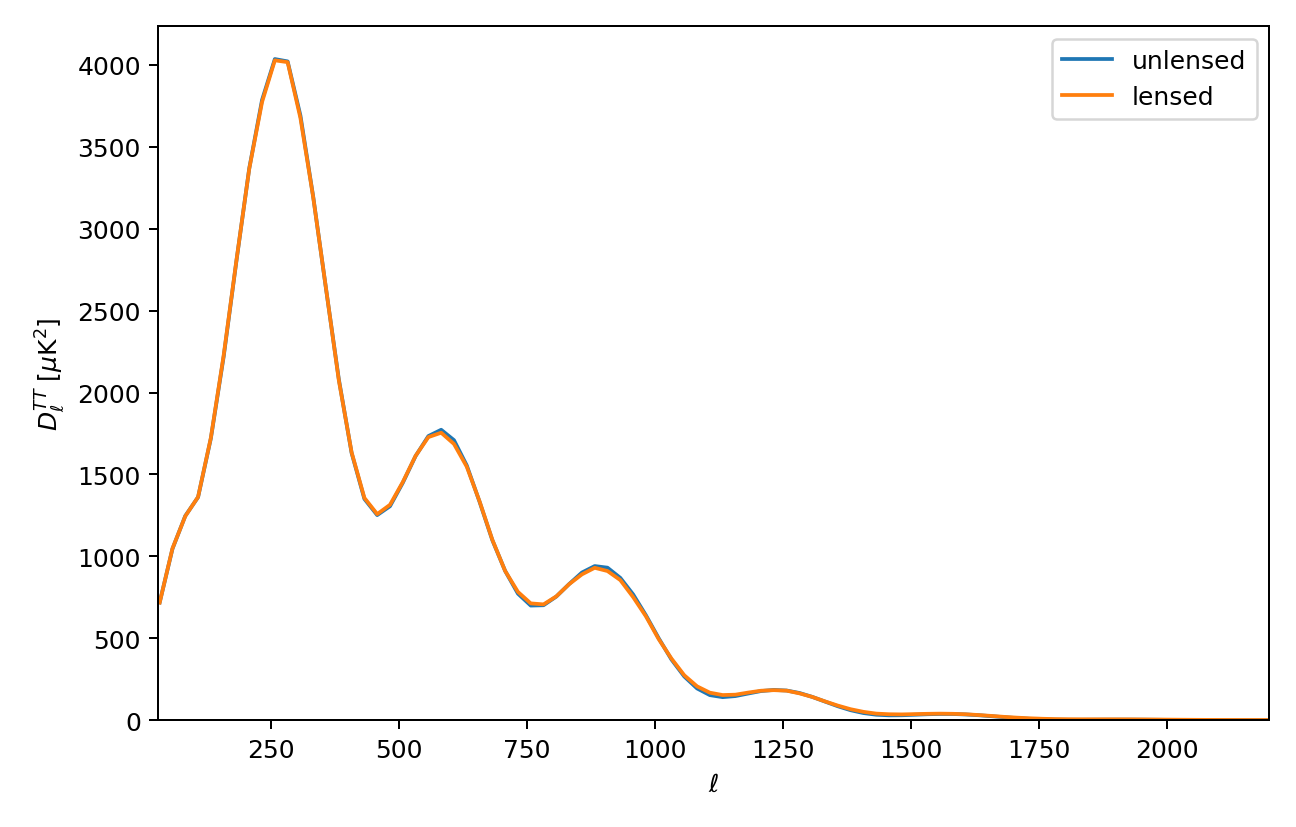
\includegraphics[width=0.88\textwidth]{figures/lens/lensed_temperature_spectrum.png}
\caption{Unlensed and lensed controlled temperature templates.  The remapping reduces acoustic contrast and transfers power into the damped high-$\ell$ tail.}
\label{fig:lensed-temperature}
\end{figure}

Selected remapped values are
\begin{center}
\begin{tabular}{rrrrr}
\toprule
$\ell$ & $D_\ell^{TT,{\rm unl}}$ & $D_\ell^{TT,{\rm len}}$ & $D_\ell^{EE,{\rm len}}$ & $D_\ell^{BB,{\rm len}}$\\
& $[\mu{\rm K}^2]$ & $[\mu{\rm K}^2]$ & $[\mu{\rm K}^2]$ & $[\mu{\rm K}^2]$\\
\midrule
$108$  & $1361.5425$ & $1362.8868$ & $0.21436$ & $8.5890\times10^{-4}$\\
$258$  & $4035.0350$ & $4027.3441$ & $0.51018$ & $5.3587\times10^{-3}$\\
$508$  & $1449.1799$ & $1453.8814$ & $5.91811$ & $1.29145\times10^{-2}$\\
$1008$ & $500.9239$  & $495.4583$  & $4.69624$ & $1.42386\times10^{-2}$\\
$1508$ & $33.8350$   & $37.7772$   & $1.46534$ & $7.5177\times10^{-3}$\\
$2008$ & $2.31049$   & $3.99422$   & $0.06954$ & $4.1477\times10^{-3}$\\
\bottomrule
\end{tabular}
\end{center}

\section{Scalar lensing \texorpdfstring{$B$}{B} mode}

The generated lensing $B$ template peaks near the acoustic-to-damping transition.  In the principal realization,
\begin{equation}
 \boxed{
 D_{1008}^{BB,{\rm lens}}
 =1.4238587\times10^{-2}\ \mu{\rm K}^2,
 }
 \label{eq:lens-bb-1000}
\end{equation}
\begin{equation}
 \boxed{
 D_{2008}^{BB,{\rm lens}}
 =4.1477498\times10^{-3}\ \mu{\rm K}^2.
 }
 \label{eq:lens-bb-2000}
\end{equation}
The refinement-to-cold ratios are
\begin{equation}
 \frac{D_{1008,D}^{BB}}{D_{1008,{\rm c}}^{BB}}
 =0.9997167797,
 \qquad
 \frac{D_{2008,D}^{BB}}{D_{2008,{\rm c}}^{BB}}
 =0.9990054398.
 \label{eq:lens-bb-ratios}
\end{equation}
Thus the benchmark predicts an ordinary-looking scalar lensing $B$ mode over the main CMB range, despite the much stronger cutoff in sufficiently small-scale low-redshift structure.

\begin{figure}[htbp]
\centering
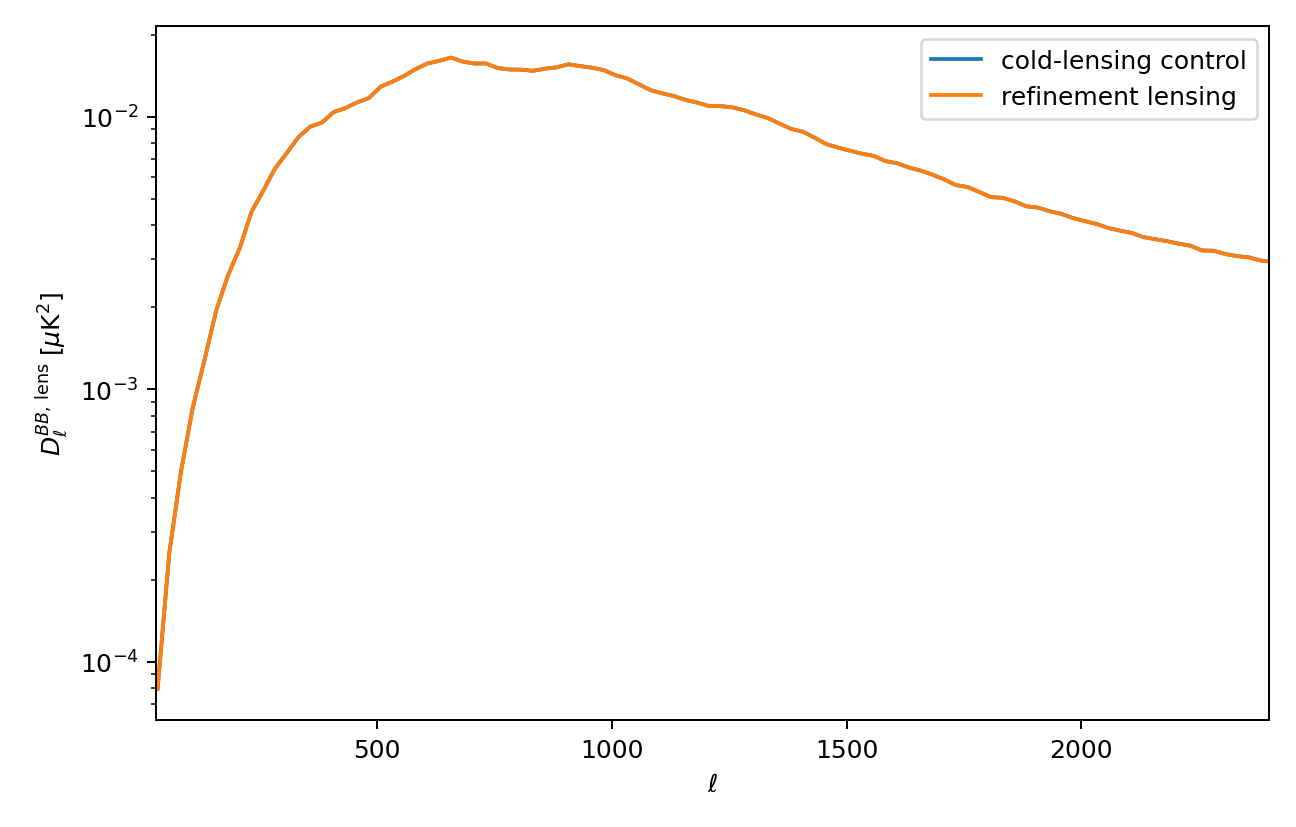
\includegraphics[width=0.86\textwidth]{figures/lens/lensing_b_modes.png}
\caption{Lensing-generated scalar $B$-mode templates.  The two curves are nearly coincident because the CMB lensing kernel mainly samples wavenumbers below the refinement half-mode scale.}
\label{fig:lensing-bmodes}
\end{figure}

\section{Cross-observable scale separation}

The CMB convergence-power ratios are
\begin{equation}
 \frac{C_{1000,D}^{\kappa\kappa}}
 {C_{1000,{\rm c}}^{\kappa\kappa}}
 =0.9993089943,
 \label{eq:lens-kappa-ratio-1000}
\end{equation}
\begin{equation}
 \frac{C_{3000,D}^{\kappa\kappa}}
 {C_{3000,{\rm c}}^{\kappa\kappa}}
 =0.9950809554,
 \qquad
 \frac{C_{5000,D}^{\kappa\kappa}}
 {C_{5000,{\rm c}}^{\kappa\kappa}}
 =0.9874740972.
 \label{eq:lens-kappa-ratio-high}
\end{equation}
The prior linear galaxy-lensing calculation gives, for a source at $z_s=0.5$,
\begin{equation}
 \frac{C_{5000,D}^{\kappa\kappa}(z_s=0.5)}
 {C_{5000,{\rm c}}^{\kappa\kappa}(z_s=0.5)}
 =0.7021280719.
 \label{eq:lens-galaxy-ratio}
\end{equation}
The same microscopic transfer therefore produces a scale- and kernel-dependent hierarchy:
\begin{equation}
 \boxed{
 \text{primary CMB lensing: nearly cold}
 \quad\text{while}\quad
 \text{low-redshift high-}\ell\text{ lensing: strongly suppressed}.
 }
 \label{eq:lens-scale-separation}
\end{equation}
The reason is geometric.  At fixed angular multipole, a lower-distance kernel probes larger physical wavenumber $k\simeq(L+1/2)/\chi$, and therefore reaches the refinement cutoff earlier.

\begin{figure}[htbp]
\centering
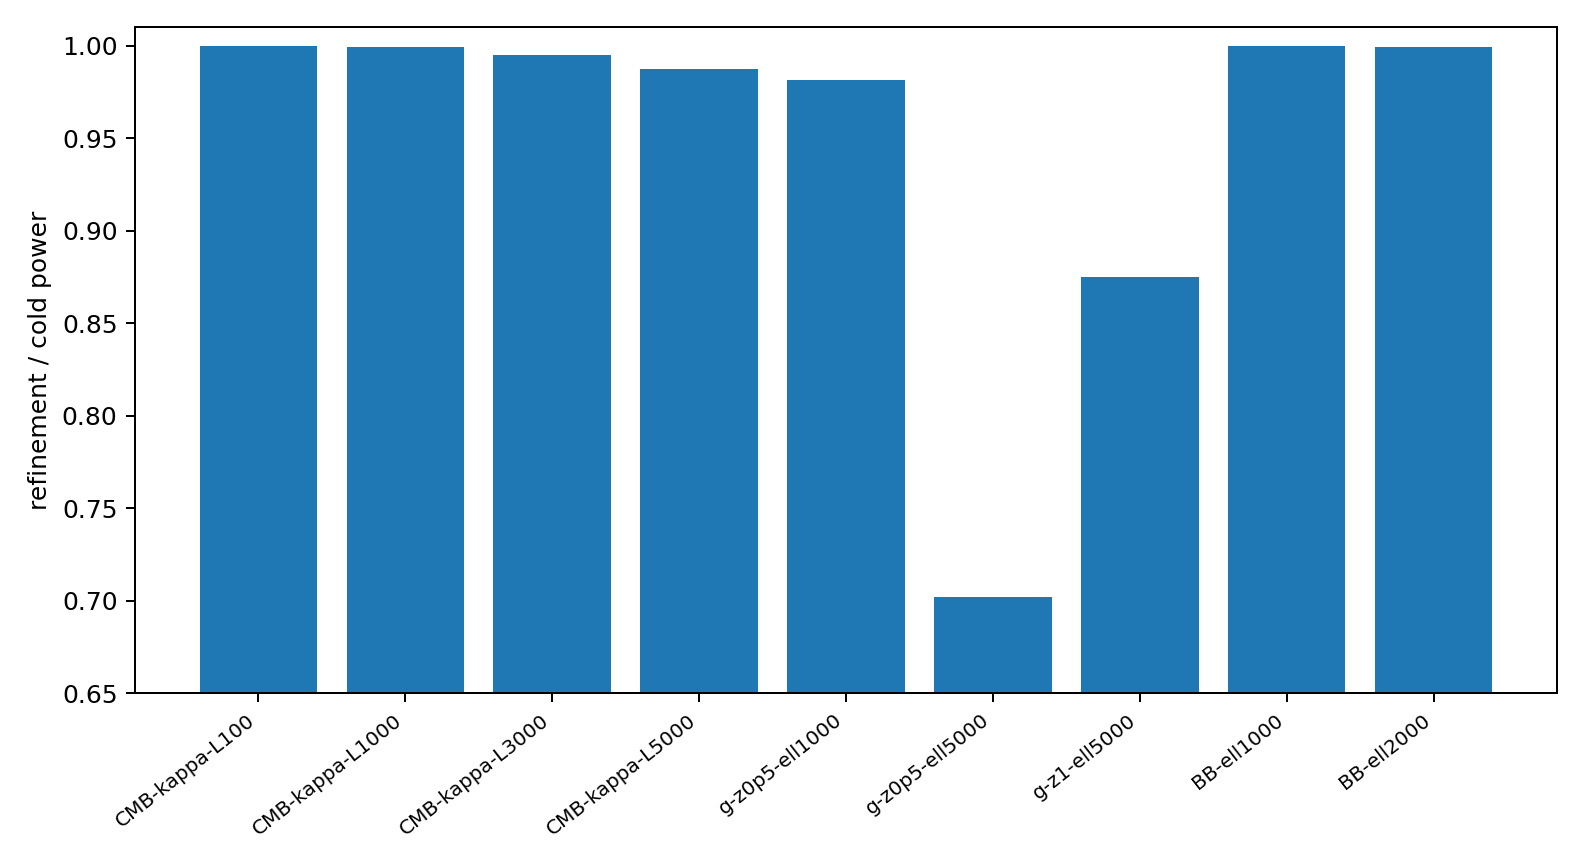
\includegraphics[width=0.94\textwidth]{figures/lens/cross_observable_scale_separation.png}
\caption{Linked lensing observables generated from the same refinement transfer.  The strong low-redshift suppression coexists with percent-level or smaller CMB-lensing corrections.}
\label{fig:lens-cross-observable}
\end{figure}

\section{Verification and convergence}

The deterministic audit records
\begin{equation}
 \boxed{
 20\ {\rm PASS},
 \qquad
 0\ {\rm FAIL}.
 }
 \label{eq:lens-pass-count}
\end{equation}
The principal controls are
\begin{center}
\begin{tabular}{lr}
\toprule
control & residual or discrepancy\\
\midrule
$\sigma_8$ reconstruction & $1.11\times10^{-16}$\\
finite-box cold deflection variance & $5.62\times10^{-4}$\\
finite-box refinement deflection variance & $5.62\times10^{-4}$\\
24-to-48 realization refinement & $1.694\times10^{-2}$\\
$448^2$-to-$512^2$ grid refinement & $1.034\times10^{-1}$\\
maximum lensed $TE$ Cauchy ratio & $0.640576<1$\\
\bottomrule
\end{tabular}
\end{center}
The grid discrepancy is dominated by the lensing $B$ tail near $\ell\simeq2000$.  Temperature and $E$-mode discrepancies are substantially smaller.  The output beyond the parent acoustic range is retained as a controlled extrapolative tail rather than a precision prediction.

\section{Closure ledger}

\begin{center}
\begin{tabularx}{\textwidth}{>{\raggedright\arraybackslash}X>{\raggedright\arraybackslash}p{0.18\textwidth}>{\raggedright\arraybackslash}p{0.24\textwidth}}
\toprule
statement & status & boundary\\
\midrule
CMB convergence and lensing potential from the fixed refinement transfer & closed controlled & linear Limber and declared $\sigma_8$ normalization\\
positive-kernel suppression theorem & proved & $0\leq T_D\leq1$\\
finite-patch Gaussian deflection realization & closed controlled & periodic flat sky\\
nonperturbative Born remapping of $T,Q,U$ & closed controlled & no post-Born correction\\
scalar lensing $B$-mode template & closed controlled & no primordial tensor $B$ mode\\
linked CMB and galaxy lensing hierarchy & closed conditional & linear source kernels\\
nonlinear matter lensing & open & nonlinear power and baryonic feedback\\
precision full-sky remapping and covariance & open & production analysis code\\
observational likelihood and parameter posterior & open & data, nuisance, and covariance model\\
\bottomrule
\end{tabularx}
\end{center}

\section{Synthesis and unresolved requirements}

The scale-covariant dark sector now predicts, with one unchanged transfer function,
\begin{equation}
 \boxed{
 \begin{gathered}
 \text{matter cutoff}
 \Longrightarrow
 \text{galaxy-lensing suppression}
 \Longrightarrow
 \text{CMB lensing potential}\\
 \Longrightarrow
 \text{remapped }TT,TE,EE
 \Longrightarrow
 \text{lensing }BB
 \end{gathered}
 }
 \label{eq:lens-result-chain}
\end{equation}
The remaining observational requirements are
\begin{equation}
 \boxed{
 \begin{gathered}
 \text{nonlinear matter and halo evolution},\\
 \text{baryonic and astrophysical nuisance sectors},\\
 \text{precision full-sky CMB remapping},\\
 \text{one joint likelihood with frozen microscopic parameters}.
 \end{gathered}
 }
 \label{eq:lens-open-requirements}
\end{equation}
